\documentclass{cwru}

\title{Exploring Alternative Routes Using Multipath TCP}
\author{Stephen Brennan}
\date{August, 2017} % Graduate date
\doctype{thesis}
\degree{Master of Science}
\department{Electrical Engineering and Computer Science}

\defensedate{June 5, 2017}

\usepackage{listings}
\usepackage{graphicx}
\usepackage{color}
\usepackage{fancyvrb}
\usepackage{acro}
\usepackage{hyperref}
\definecolor{mygreen}{rgb}{0,0.6,0}
\definecolor{mygray}{rgb}{0.5,0.5,0.5}
\definecolor{mymauve}{rgb}{0.58,0,0.82}
\lstset{%
  backgroundcolor=\color{white},     % background color
  basicstyle=\footnotesize\ttfamily, % monospace, small font
  breaklines=true,                   % nice line breaks
  captionpos=b,                      % put captions at bottom
  commentstyle=\color{mygreen},      % comments
  escapeinside={(*}{*)},             % if you want to add LaTeX in code
  keywordstyle=\color{blue},         % keyword
  stringstyle=\color{mymauve},       % string
}

\DeclareAcronym{mptcp}{
  short = MPTCP,
  long  = Multipath TCP
}
\DeclareAcronym{dss}{
  short = DSS,
  long  = Data Sequence Signal
}
\DeclareAcronym{as}{
  short        = AS,
  long         = Autonomous System,
  short-plural = es
}
\DeclareAcronym{bgp}{
  short = BGP,
  long  = Border Gateway Protocol
}
\DeclareAcronym{ospf}{
  short = OSPF,
  long  = Open Shortest Path First
}
\DeclareAcronym{ron}{
  short = RON,
  long  = Resilient Overlay Network
}
\DeclareAcronym{lsrr}{
  short = LSRR,
  long  = Loose Source and Record Route
}
\DeclareAcronym{ssrr}{
  short = SSRR,
  long  = Strict Source and Record Route
}
\DeclareAcronym{sosr}{
  short = SOSR,
  long  = Scalable One-hop Source Routing
}
\DeclareAcronym{nat}{
  short = NAT,
  long  = Network Address Translation
}
\DeclareAcronym{ecmp}{
  short = ECMP,
  long  = Equal Cost Multi-Path Routing
}
\DeclareAcronym{lia}{
  short = LIA,
  long  = Linked Increase Algorithm
}
\DeclareAcronym{olia}{
  short = OLIA,
  long  = Opportunistic Linked Increase Algorithm
}
\DeclareAcronym{wvegas}{
  short = wVegas,
  long  = Delay-based Congestion Control
}
\DeclareAcronym{balia}{
  short = BALIA,
  long  = Balanced Linked Adaptation Algorithm
}
\DeclareAcronym{mcp}{
  short = MCP,
  long  = Multipath Conversion Point
}

\begin{document}
\advisor{Michael Rabinovich}
\committee{Vincenzo Liberatore}
\committee{Mark Allman}

% The organization of the dissertation must follow the order below:
%
% Title page
% Committee Approval Sheet
% Copyright page (only if copyrighting)
% Dedication page (optional)
% Table of Contents
% List of Tables
% List of Figures
% Preface (optional)
% Acknowledgements (optional)
% List of Abbreviations (optional)
% Glossary (optional)
% Abstract
% --TEXT--
% Appendix
% Bibliography

\maketitle
\makeapprovalsheet

\setcounter{tocdepth}{1}
\frontmatter
\tableofcontents

\cleardoublepage
\phantomsection
\addcontentsline{toc}{chapter}{List of Figures}
\listoffigures

%\begin{acknowledgments}
%\lipsum[1-3]
%\end{acknowledgments}

% If you're using `glossaries` package

%\cleardoublepage
%\phantomsection
%\addcontentsline{toc}{chapter}{List of Acronyms}
%\printglossary[type=\acronymtype]

%\cleardoublepage
%\phantomsection
%\addcontentsline{toc}{chapter}{Glossary}
%\printglossary

% because they were probably used above
\acresetall

\begin{abstract}
  \ac{mptcp} is an extension to TCP which allows hosts to establish connections
  consisting of multiple TCP ``subflows'' that travel across different Internet
  paths. However, it is based on the assumption that at least one communicating
  host is multi-homed. Meanwhile, the Internet contains considerable path
  diversity, and research has shown that routes chosen by the Internet are not
  always the most efficient. In this thesis, we implement and evaluate a
  mechanism which allows single-homed devices to leverage \ac{mptcp} and
  establish subflows across alternative routes. We find that this mechanism is
  capable of significant bandwidth aggregation under appropriate network
  conditions, and that the mechanism is deployable on today's Internet, for
  unmodified applications.
\end{abstract}

\mainmatter
\chapter{Introduction}

This thesis proposes a mechanism for exploring and adding alternative paths to a
\ac{mptcp} connection, for the purpose of improving application throughput.
These alternative paths travel through ``detour'' hosts, ensuring that the paths
are distinct from the Internet routed path. The bandwidth of these paths can be
aggregated, allowing better throughput than any of the constituent paths.

\section{Internet Routing Inefficiencies}

The Internet is made up of several \acp{as}, each containing many routers.
Routers forward packets along their outgoing interfaces according to an internal
routing table. This table is populated with routes learned from the external
\ac{bgp}, as well as intra-\acs{as} protocols such as \ac{ospf}. Administrators
have considerable freedom to enforce local policy on which routes to advertise,
and which routes to use. Additionally, the metrics used in route selection
include hop count and \ac{as} count, which may not correlate well with important
path characteristics such as loss rate or latency.

As a result, the default Internet path between hosts is not always the ``best
path'' with respect to these characteristics. In \cite{detour}, Savage
\textit{et al.} measured the pairwise latency and packet drop rates among a
group of hosts. From this dataset, they searched for instances where these
metrics were better along a ``detour'' route going through a third host. They
found that half of all pairs of hosts had a ``detour'' route with lower latency,
and 15\% of the pairs of hosts had a path with at least 25\% improvement in
latency. For packet loss, 80\% of the pairs had a detour path with a lower
packet loss rate, and in nearly half, the packet loss rate improved by a factor
of six.

Overlay networks have been proposed as a way to experiment with new routing
techniques. These techniques create a second network on top of the existing
Internet. Peers in these overlays are connected by \textit{virtual links}, which
are simply routes in the underlying Internet. Packets are tunneled from peer to
peer until reaching their end destination. Overlay networks like these have been
shown to improve on path metrics like throughput and loss rates
\cite{detour,ron}.

\section{Access Link Underutilization}

With the advent of fiber-to-the-home connections, residential access link speeds
have been increasing. While conventional wisdom has been that access links are
usually the bottleneck, this is not always the case \cite{akella2003empirical}.
While they have increased, studies have shown that residential link bandwidths
are not fully utilized, especially fiber connections \cite{fibertothehome}.
There are many reasons why this is this is the case. For one, short-lived TCP
connections may never leave the slow start phase. For another, TCP initial
window settings may not be high enough to accommodate faster links. However,
sometimes the default Internet route may not be able to accommodate these higher
speeds.

With alternative routes available that may perform better, it makes sense to
explore these alternative routes. Rather than selecting a single path, it also
makes sense to use both simultaneously, aggregating their available throughput.

\section{Contributions}

\begin{figure}
  \centering
  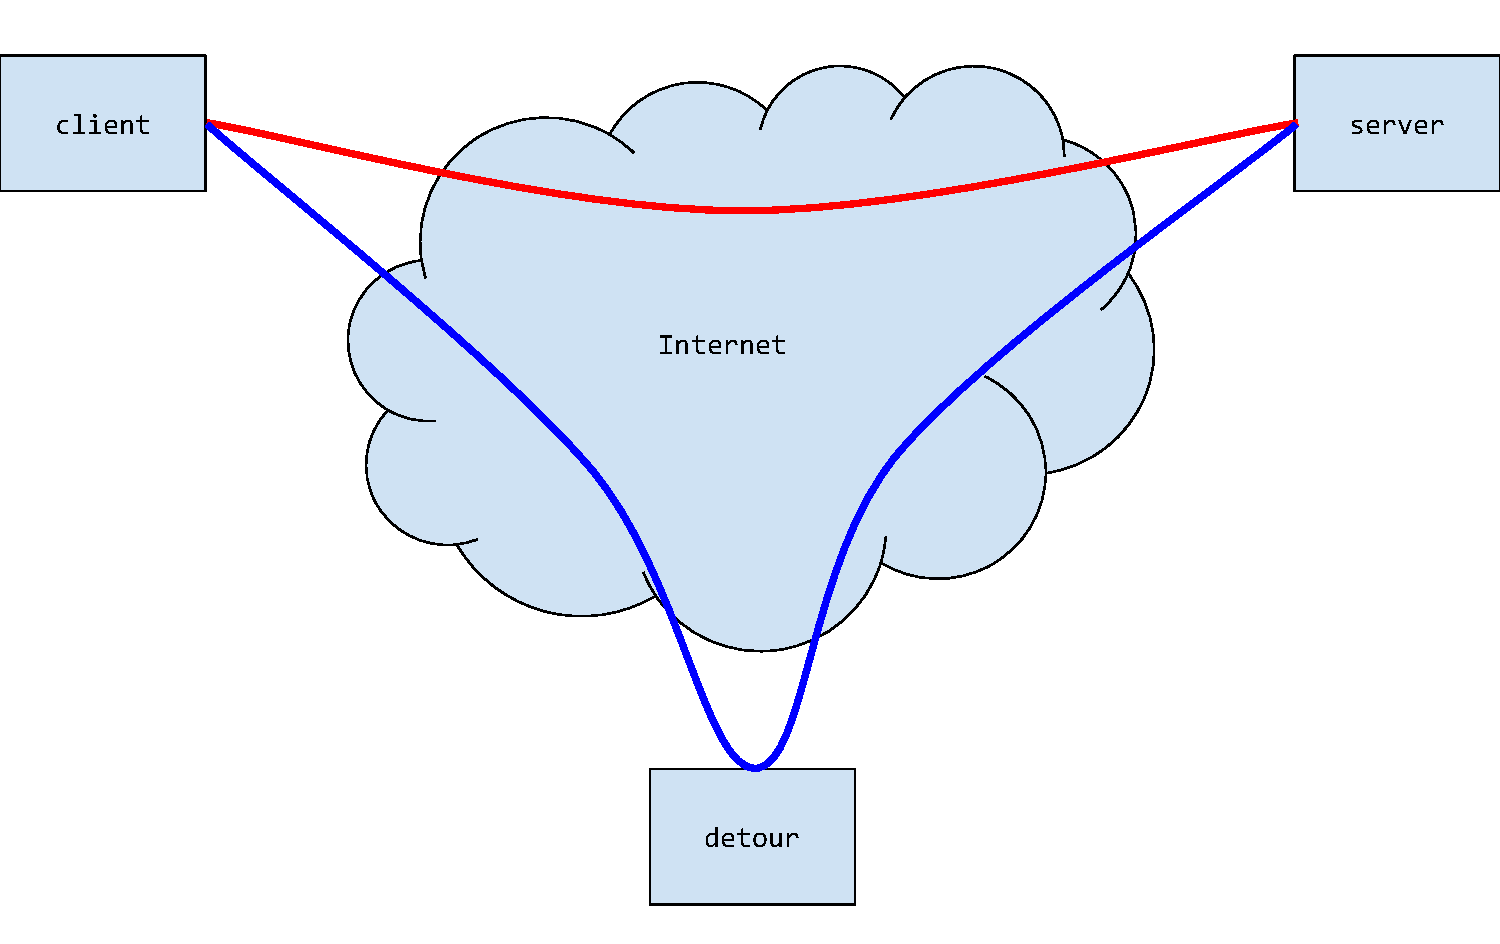
\includegraphics[width=0.8\textwidth]{figures/Concept.pdf}
  \caption{Conceptual overview of the mechanism}
  \label{fig:concept}
\end{figure}

This thesis presents a mechanism for single-homed devices to add alternative
paths that traverse third-party ``detour'' hosts. This mechanism, illustrated in
Figure~\ref{fig:concept} is based on \ac{mptcp}, establishing subflows through
each alternative route. Using \ac{mptcp} allows multiple routes to be used for a
single connection, with data divided across each route. Additionally, since
\ac{mptcp} uses the same binary-compatible OS level API as TCP, unmodified
applications may use this mechanism simply by using our patched kernel.

The contributions of this thesis are as follows:
\begin{itemize}
\item A system of Linux kernel modifications and user-space tools that allow
  alternative routes to be added to \ac{mptcp} connections.
\item An evaluation of the method on emulated and real world networks.
\end{itemize}

The remainder of this thesis will follow the following structure. Background
information on \ac{mptcp} and the mechanisms used in the evaluation is covered
in Chapter~\ref{c:bg}. Related work is discussed in Chapter~\ref{c:rw}. The
implementation of our system is described in Chapter~\ref{c:impl}. Experimental
evaluation is presented in Chapter~\ref{c:eval}. Finally, future work is
discussed in Chapter~\ref{c:fw} and we conclude in Chapter~\ref{c:conclusion}.

\chapter{Background}
\label{c:bg}

\section{Multipath TCP}
% Our discussion of Multipath TCP needs to be in enough depth that the reader
% understands how it works - essentially covering at least the first few pages
% of the RFC. In particular:
% - Subflows: what they are and how they work
% - How the initial subflow is created
% - How subsequent subflows are created and authenticated
% - Data sequencing and how data sequences are mapped onto subflow sequences
% - path management and data scheduling
% - ? how the linux kernel implementation is structured

Recently, multi-homed devices have become increasingly common. The most obvious
example of these devices is the smartphone, which typically comes with at least
two network interfaces: one for cellular data, and one for Wi-Fi. While these
devices have become more common, protocols have not kept up. Most Internet
traffic is carried on TCP, which identifies a data stream by the 5-tuple of
protocol, source address and port, and destination address and port. As a
result, multi-homed devices are forced to choose only one interface for a TCP
session \cite{raiciu2012hard}. \ac{mptcp} was designed as a protocol extension
to TCP, which allows multiple interfaces (and as a result, network paths) to be
used in the same TCP stream.

\subsection{Design Considerations}

\ac{mptcp} has several design goals, outlined in \cite{rfc6182}. At a high
level, it aims to use the existence of multiple paths to improve efficiency and
resiliency of standard TCP. Other transport protocols support this, such as SCTP
with Concurrent Multipath Transfer \cite{iyengar2006concurrent}. However, SCTP
cannot easily be used as a replacement for TCP, because applications would
require modification, and some NATs and firewalls do not support SCTP
\cite{barre2011multipath}. As a result, \ac{mptcp} also aims to be compatible
with the Internet today, so it can be deployed widely.

\ac{mptcp}'s design focuses on two types of compatibility, which motivate many
of its high-level design decisions. First, application compatibility: \ac{mptcp}
must be usable by existing TCP applications without modification. Second,
network compatibility: \ac{mptcp} must be usable across the Internet today,
including across features of the modern Internet such as NAT, firewalls, traffic
normalizers, and performance-enhancing proxies (collectively referred to as
middleboxes). In the design of \ac{mptcp}, consideration is made for the
following types of disruption by middleboxes \cite{rfc6182}:

\begin{itemize}
\item Home routers often perform NAT, and so addresses may not be the same on
  either side of a connection.
\item Some NAT boxes will additionally rewrite content of some protocols, such
  as URLs in HTTP \cite{rfc6182} and IP addresses and ports in FTP
  \cite{raiciu2012hard}.
\item Some middleboxes perform sequence number randomization.
\item Some middleboxes strip unrecognized options from packets.
\item Some middleboxes (especially traffic normalizers) will not allow ``holes''
  in TCP sequence numbers.
\item TCP segments may be broken up (for example, segmentation offload) or
  coalesced. TCP options on these segments must be constructed in a way that
  this process will not make the data uninterpretable.
\end{itemize}

Finally, an additional network compatibility requirement is that \acl{mptcp}
``do no harm'' to existing TCP flows \cite{rfc6182}. As a result, several
congestion control mechanisms are proposed, aiming to prevent \ac{mptcp} from
using more resources than a single TCP flow would across a shared bottleneck
\cite{rfc6356,draft-olia,draft-balia,draft-wvegas}.

These combined architectural guidelines not only make \ac{mptcp} suitable for
deployment, but they also make it more resilient to the mechanisms used in this
thesis (such as NAT) to extend it in new ways.

\subsection{Architecture}

\begin{figure}[h]
  \centering
\begin{BVerbatim}
                             +-------------------------------+
                             |           Application         |
+---------------+            +-------------------------------+
|  Application  |            |             MPTCP             |
+---------------+            + - - - - - - - + - - - - - - - +
|      TCP      |            | Subflow (TCP) | Subflow (TCP) |
+---------------+            +-------------------------------+
|      IP       |            |       IP      |      IP       |
+---------------+            +-------------------------------+
\end{BVerbatim}
\caption[Comparison of TCP and \acs{mptcp} Protocol Stacks]{Comparison of
  Standard TCP and \ac{mptcp} Protocol Stacks. Originally from \cite{rfc6824}}
  \label{fig:layers}
\end{figure}

To achieve these goals, \ac{mptcp} is located between TCP and the application
layer, as shown in Figure~\ref{fig:layers}. While a naive approach would simply
send different segments on different paths, this would create ``sequence
number holes'' from the perspective of middleboxes \cite{raiciu2012hard}. To
remain compatible, a ``subflow'' is created along each path. Each subflow looks
like a normal TCP connection, but with some additional options, and slightly
different semantics.

A \ac{mptcp} connection begins with a three-way handshake, similar to a regular
TCP connection. If both hosts are capable and willing to use \ac{mptcp}, they
include a TCP option with subtype \texttt{MP\_CAPABLE} on all packets of the
handshake. Additional TCP connections (referred to as ``subflows'') may be
created between the two hosts once the initial one is established, using the
\ac{mptcp} option subtype \texttt{MP\_JOIN}. To authenticate this process, keys
are exchanged via the \texttt{MP\_CAPABLE} option, and a token is verified using
these keys for each new subflow via the \texttt{MP\_JOIN} option.

An implementation may establish a new subflow with its peer at any time
according to local policy. Additional addresses may be explicitly advertised
using the \ac{mptcp} option subtype \texttt{ADD\_ADDR}, and they may be removed
via the \ac{mptcp} option subtype \texttt{REMOVE\_ADDR}. These options are not
reliably transmitted, so they are purely informational. While either side of a
connection may initiate a new subflow, it is expected that the client (i.e.
active opener) initiate most subflows, due to firewalls and NAT.

Data has sequence numbers at both the subflow level and at the connection level.
Each subflow has a \ac{dss} negotiated via the \ac{mptcp} option subtype
\texttt{DSS}, which maps subflow sequence numbers to data sequence numbers.
These mappings are valid for only a certain amount of bytes, and thus new
mappings must be transmitted periodically. As a result, the \ac{dss} is one
persistent form of overhead in the protocol header. Data is acknowledged both
at the subflow level (via the \texttt{ACK} flag), and at the data level (via a
flag within the \ac{dss}).

\subsection{Implementation}

\ac{mptcp} is implemented in the Linux kernel, as well as within the XNU kernel
used by Mac OS and iOS. In this thesis, we focus on version 0.91 of the Linux
kernel implementation \cite{mptcp}. This implementation has three key features
which enable flexibility and custom policy: data schedulers, congestion control,
and path managers.

As a result of \ac{mptcp}'s flexibility in labeling data with sequence numbers,
data may be split up across multiple subflows, or even transmitted redundantly.
A data scheduler is a modular component which determines which subflow to send
application data on. The default scheduler implementation, Lowest RTT First,
selects the subflow with the smallest RTT and fills up its congestion window.
Other implementations include a naive round-robin scheduler and one which sends
data redundantly across each subflow. Additional schedulers have been proposed,
to mitigate problems such as head-of-line blocking and bufferbloat
\cite{paasch2014experimental}. In this thesis, we consider only the Lowest RTT
First scheduler.

As with regular TCP congestion control, \ac{mptcp} congestion control is
implemented as a modular component of the Linux kernel. While normal TCP
congestion control algorithms (such as the Linux default, CUBIC) may be used on
each subflow, several \ac{mptcp} specific implementations are provided: \ac{lia}
\cite{rfc6356}, \ac{olia} \cite{draft-olia}, \ac{wvegas} \cite{draft-wvegas},
and \ac{balia} \cite{draft-balia}. In this thesis, we only consider \ac{lia}
congestion control.

In order to decide when to create and destroy new subflows, as well as advertise
alternative addresses, the Linux implementation uses another modular component
called a ``path manager'' \cite{mptcp}. The default implementation does nothing
(except accepting incoming connections). The Linux implementation also includes
an \texttt{ndiffports} path manager, which initiates up to $N$ subflows with a
server, from different source ports. This path manager can be useful for
\ac{ecmp}, which will be discussed shortly. A \texttt{fullmesh} path manager
establishes subflows between every pair of client addresses and advertised
server addresses. A major part of the implementation of this thesis is a path
manager for the Linux kernel \ac{mptcp} implementation.

% Netfilter and Netlink?
% OpenVPN?

\section{Mininet}

In the evaluation of our mechanism, we use the Mininet \cite{mininet} framework
to emulate a network topology and evaluate performance across the emulated
network. Although this framework is not new in the literature of \ac{mptcp}
measurement studies \cite{paasch2013benefits,paasch2014experimental}, we use
this section to give a brief overview of its operation.

Mininet is a software-defined networking tool that allows the creation of
virtual networks. Networks created within Mininet use the native OS network
stack, and can run applications unmodified using the virtual network. However,
they do not require the full overhead of virtual machines, which emulate an
entire guest operating system and any virtual hardware used by the guest.
Instead, Mininet nodes are simply process groups using the host operating system
to access either real network devices, or virtual ones.

Mininet works by leveraging the lightweight virtualization mechanisms that the
Linux kernel provides. Within the kernel, \emph{namespaces} are used to organize
and partition the resources a process (or group of processes) can see and use.
For instance, mount namespaces limit an application's view of the file system.
PID namespaces give a group of applications a new set of process identifiers,
starting from 1. Similarly, network namespaces group the resources of the
operating system network stack. In particular, network namespaces group network
interfaces, as well as routing tables and firewall rules. Kernel namespaces are
the foundation of modern lightweight virtualization tools such as Docker.

Network namespaces may be connected by virtual Ethernet pairs, such that traffic
sent on a virtual interface on within one namespace can be received on a virtual
interface within another. Furthermore, these virtual Ethernet links may be
configured using the Linux Traffic Control framework, to emulate packet loss,
latency, jitter, reordering, retransmission, and control link bandwidth.

Mininet creates virtual networks via the following mechanism
\cite{lantz2010network}. Each host is a shell process running within a separate
network namespace. Hosts share a pipe to the Mininet parent process, over which
commands and output are exchanged. Links are virtual Ethernet pairs. Switches
may be emulated using userspace or kernel OpenFlow switch implementations,
although we did not use switches in our experiments.

As a network emulation framework, Mininet presents several attractive qualities.
It is more lightweight than virtual machines, enabling practical experimentation
on single machines. It provides an easy-to-use Python API, reducing manual
interaction in the experimentation process. By providing complete virtual
machine images with Mininet and experiments pre-installed, experiments may be
made completely reproducible, and distributed easily online. Finally, as
compared to larger, hardware based emulation frameworks such as EmuLab, the
development time and debugging time can be dramatically reduced when developing
experiments.

\chapter{Related Work}
\label{c:rw}

The mechanism in this thesis involves adding alternative routes to a connection,
in order to improve connection performance. This can be seen as related to
several concepts in the body of networking research: multipath routing, overlay
routing, source routing, channel bonding, and proxying. In this chapter, we will
examine related work at each relevant level of Internet.

\section{Link Layer}
\label{s:rw-ll}

At the link layer, aggregating multiple low-capacity links to create a single,
virtual link with higher capacity is called \emph{inverse multiplexing}, or
sometimes channel bonding \cite{duncanson1994inverse}. Linux provides a bonding
driver which allows this to be done in software, presenting a single virtual
interface to the host machine. Unfortunately, this mechanism typically requires
identical links and configuration on either side of them, limiting the use of
these setups \cite{chiussi1998generalized}.

Another interesting approach to bandwidth aggregation, falling somewhere between
the link layer and the network layer, is the ``Beyond One's Bandwidth (BOB)''
system \cite{radio-agg}. This system, designed for use on residential wireless
access points, allows neighboring residential access points to share bandwidth.
Each router negotiates a connection with its neighboring access points, and uses
round-robin scheduling to assign packet flows to different gateways. Streams,
like TCP, must remain on the gateway that their initial packet used, so the
system does not truly aggregate bandwidth for streams. The authors considered
implementing a \ac{mptcp} proxy with subflows over each gateway, but rejected
this strategy since it required an egress point on the wide area Internet.

\section{Network Layer}

Improved Internet routing has been a goal for researchers for a long time, and
the network layer has been a natural place to begin. Related work on the network
includes source routing, overlay routing schemes, and several multipath routing
approaches.

\subsection{Source Routing}

A major part of this thesis (and many other studies) involves specifying
``waypoints'' or detour hosts that a packet must traverse before it continues on
to its final destination. Although packets are normally routed on the Internet
hop-by-hop, there are mechanisms for specifying the path that a packet should
take. In IPv4, these mechanisms are the options \ac{lsrr} and \ac{ssrr}
\cite{rfc791}. These IP options allow the source of a packet to specify a
partial (Loose) or complete (Strict) route consisting of a list of addresses. In
IPv6, a similar mechanism called Segment Routing is being proposed by the IPv6
Maintenance Working Group of the IETF \cite{draft-segment-routing}. Options like
these are most useful within a single managed system, since they are not
respected on the wide area Internet, due to the potential for spoofing IP
addresses while still receiving reply packets.

\subsection{Overlay Routing}

Beyond Source Routing, there are no mechanisms to experiment with how routers
work on the Internet. As the IPv6 deployment process has demonstrated, network
layer protocols are not easy to change.

An alternative to designing and deploying a full new network layer protocol is
experimenting on overlay networks. Overlay networks are networks constructed on
top of an existing ``substrate'' network. Nodes route traffic among each other
using the substrate network rather than direct links. Traffic is routed through
a sequence of overlay nodes before reaching the final destination, rather than
being directly routed through the substrate. In the case of the Internet, these
networks can be advantageous because they can add functionality that is not
widely deployed (such as multicasting) and they can make routing decisions based
on more information than the Internet.

Several overlay network approaches have been proposed and deployed. An early
example, the M-Bone, connected networks capable of multicasting via tunnels
\cite{mbone}. This allowed multicasting even though the Internet as a whole did
not support it. Later approaches, such as Overcast \cite{jannotti2000overcast},
apply the concept of overlay networking at the application level to achieve
similar results.

In \cite{ron}, Andersen \textit{et al.} described \ac{ron}, a framework for
creating overlay networks and routing traffic along them. Applications link to a
user-space library, and access the network via a \texttt{send} function and a
\texttt{recv} callback. Applications may choose to send via the default Internet
routed path, or via the overlay. Routing is performed at each node, rather than
at the source. The routing algorithm takes into account several virtual link
characteristics, as well as application-specified metrics, which are stored in a
database.

The design goal of \ac{ron} is to improve reliability by using overlays. The
result also showed that latency and throughput could be improved via overlays.
However, as an application-level approach, \ac{ron} cannot be applied to
unmodified applications. In \cite{andersen2003best}, Andersen \textit{et al.}
later described a redundant routing scheme in which redundant copies of packets
are sent along multiple paths. They compared this approach with a more
traditional approach that reacts to link failures and routes around them,
similar to the \ac{ron} framework's original routing system. However, they did
not attempt to use multiple paths without redundancy, since their study focused
on loss rates rather than throughput.

Another extension of the \ac{ron} framework attempted to use a biologically
inspired approach to multi-path routing \cite{leibnitz2006biologically}. Their
mechanism discovers routes via an iterative broadcasting method, not unlike the
construction of a shortest path tree. When a selection of routes is ready, the
mechanism moves into a route maintenance mode. A main route is selected, with
alternative routes being used as backups. Based on changes in link state, as
well as some degree of randomness, the main route may become backup, while a
different route is selected as the main route. As a result, this mechanism does
not appear to achieve a high degree of aggregation.

Gummadi \textit{et al.} \cite{gummadi2004improving} demonstrated a simpler
approach to detour routing. Rather than creating a full overlay network in which
each node monitors links and maintains routing tables, they applied source
routing. They designed \ac{sosr}, a system which tunnels traffic to an
intermediary, which then forwards the traffic on to the destination. The
intermediary performs \ac{nat}, so that reply traffic is forwarded back to the
destination. Using \ac{sosr} and randomly selected PlanetLab intermediaries,
they were able to recover from 56\% of failures on the paths to popular web
servers. However, they did not report the throughput of \ac{sosr} paths. In this
thesis, we use an approach very similar to Gummadi \textit{et al.} in simply
tunneling traffic across a chosen intermediary, rather than constructing a
complete overlay network.

As far as we could find, there are no overlay routing systems which attempt to
correct Internet routing inefficiencies by combining multiple paths without
redundancy. However, transport-layer systems based on overlay networks have been
created which do so (see Section~\ref{s:rw-transport}).

\subsection{Equal Cost Multi-path Routing}

The \ac{mptcp} protocol specification specifically allows for subflows to be
established from the same client address, to the same server address, with
simply a different source port \cite{rfc6824}. One reason this is allowed is to
enable path diversity via \ac{ecmp}. In large data center networks, highly
redundant network topologies have been deployed, so that there are several
routes between hosts. Such routing topologies use \ac{ecmp} to choose between
paths that have the same cost, by using a hash of the connection 5-tuple
\cite{raiciu2011improving}. In \cite{raiciu2011improving}, Raiciu \textit{et
  al.} describe in detail a simulation study that evaluates the performance of
\ac{mptcp} on several data center topologies and congestion controls. They also
describe a validation on an Amazon EC2 data center with a highly redundant
topology, in which using \ac{mptcp} with four subflows achieved a 3x throughput
improvement.

\subsection{Binder}

Another application of \ac{mptcp} to bandwidth aggregation is Binder, a system
for aggregating the bandwidth of several Internet gateways \cite{binder}. This
mechanism was developed in an area of rural Scotland, containing several
low-bandwidth gateways. Rather than use one gateway primarily and others as
backup, Binder allows aggregation of all of the gateways.

This is achieved by routing all outgoing traffic through an OpenVPN connection.
The OpenVPN connection uses \ac{mptcp}. One subflow is dedicated to each gateway
(using IP source routing options). The OpenVPN server, located outside of the
local network, terminates the \ac{mptcp} connection and performs \ac{nat},
routing all packets to their final destinations.

We consider this to be a network layer mechanism since it forwards IP datagrams
over the OpenVPN connection. As pointed out in their paper, Binder strikingly
parallels channel-bonding techniques such as the ones described in
Section~\ref{s:rw-ll}.

Our mechanism also uses OpenVPN, but a key differentiation is that while Binder
uses OpenVPN over \ac{mptcp}, we only put a single subflow of an \ac{mptcp}
connection through OpenVPN.

\section{Transport Layer}
\label{s:rw-transport}

\ac{mptcp}, the heart of our mechanism, is at the transport layer. It is built
on several years of research and development, and the literature is full of work
related to the development of multipath transport algorithms. Overviews of these
prior works can be found in \cite{barre2011multipath,raiciu2012hard}. Most of
these works are based on multi-homed devices, and thus not directly related to
this thesis.

However, one prior transport-layer approach is very relevant. In
\cite{zhang2004transport}, Zhang \textit{et al.} describe the implementation of
mTCP, an early multipath variation of TCP. Rather than using a TCP connection
per-subflow, mTCP simply routes TCP segments across different paths. Congestion
control is performed separately on each ``subflow'', while the receive window is
global. Acknowledgements are transmitted on only one return path.

Paths are dynamically added based on a heuristic that involves an estimated path
disjointness metric based on traceroute and latency. Paths are suppressed when
shared congestion is detected, and removed if they are detected to have failed.

The mTCP mechanism is based on a user-space TCP implementation, and it uses
\ac{ron} \cite{ron} as the network-layer which provides multiple routes. As a
result, the mechanism is not directly deployable on the Internet, nor could it
be easily made compatible with existing applications. In the years since mTCP
was designed, \ac{mptcp} was designed and overlay networks have become less
common. We view this thesis as a modern, compatible, and deployable take on the
concepts in mTCP.

\section{Application Layer}

At the application layer, a recent \ac{mptcp} IETF working group draft proposes
a set of proxying mechanisms that allow ISPs to improve client TCP and
\ac{mptcp} connection throughput \cite{boucadair-mptcp-plain-mode-10}. Based on
observations that \ac{mptcp} server deployment has not been strong, these
mechanisms expect a server and optionally a client which do not support
\ac{mptcp}. They proxy traffic through \acp{mcp}, devices which ISPs deploy
throughout the network. There are two possible deployment scenarios: one
\ac{mcp} and two \ac{mcp}.

In the one \ac{mcp} scenario, an \ac{mptcp}-enabled client would like to use
\ac{mptcp} to connect to a server which does not support it. It establishes a
connection to a \ac{mcp}, specifying the final destination within the
\texttt{SYN} segment. It may then establish additional subflows to the \ac{mcp}
using its other interfaces. The \ac{mcp} proxies the connection data to the
final destination via a plain TCP connection.

In the two \ac{mcp} scenario, both the client and server are not \ac{mptcp}
enabled. Instead, a TCP connection bearing an \texttt{MP\_CONVERT} TCP option is
routed through the ISP, to an \ac{mcp}. The \ac{mcp} establishes a \ac{mptcp}
connection to another \ac{mcp}, which will then connect to the final destination
over TCP.

These mechanisms are at the application layer, because they terminate TCP and
\ac{mptcp} connections, acting as proxies.

\chapter{Implementation}
\label{c:impl}
% Section intro:
% 1. Expectations (what hosts are there, and which ones run our code?)
% 2. Overview of the distinct pieces of software (client kernel, client daemon,
%    detour daemon)
% Subsection - Detour daemon
% Subsection - Client kernel
% Subsection - Client daemon

% smoother transition once we have everything

In this project, we implement a system which allows one host to dynamically add
new overlay routes to a Multipath TCP connection. Each overlay route is a new
subflow, which is tunneled across a third-party host. The system involves at
least three hosts:
\begin{itemize}
\item The \emph{client} is the active opener of the \ac{mptcp} connection. In
  our system, the client actively requests all detours and initiates all
  subflows.
\item The \emph{server} is the passive opener of the \ac{mptcp} connection.
\item The \emph{detour} is a host which acts as a waypoint along the overlay
  route from the client to the server. There may be more than one detour at a
  time, and there are multiple ways to implement the detour service.
\end{itemize}

We assume that the server supports Multipath TCP, and require no additional
customization for our system to work. In our current implementation, the detour
host must run some version of Linux, and the client must run a version of the
Linux kernel that is built with support for \ac{mptcp} and our path manager
patch.

The system is implemented via a number of interacting components. First, a path
manager extension for version 0.91 of the Linux \ac{mptcp} implementation
\cite{mptcp}, which allows the client's kernel to request new detour paths,
receive them, and create subflows across them. Second, a user-space utility
which receives messages from the kernel and creates the necessary detour paths.
Finally, we implement two different types of detour daemons, which run on the
detour host. These components are illustrated in Figure~\ref{f:MovingParts}.

\begin{figure}[h]
  \centering
  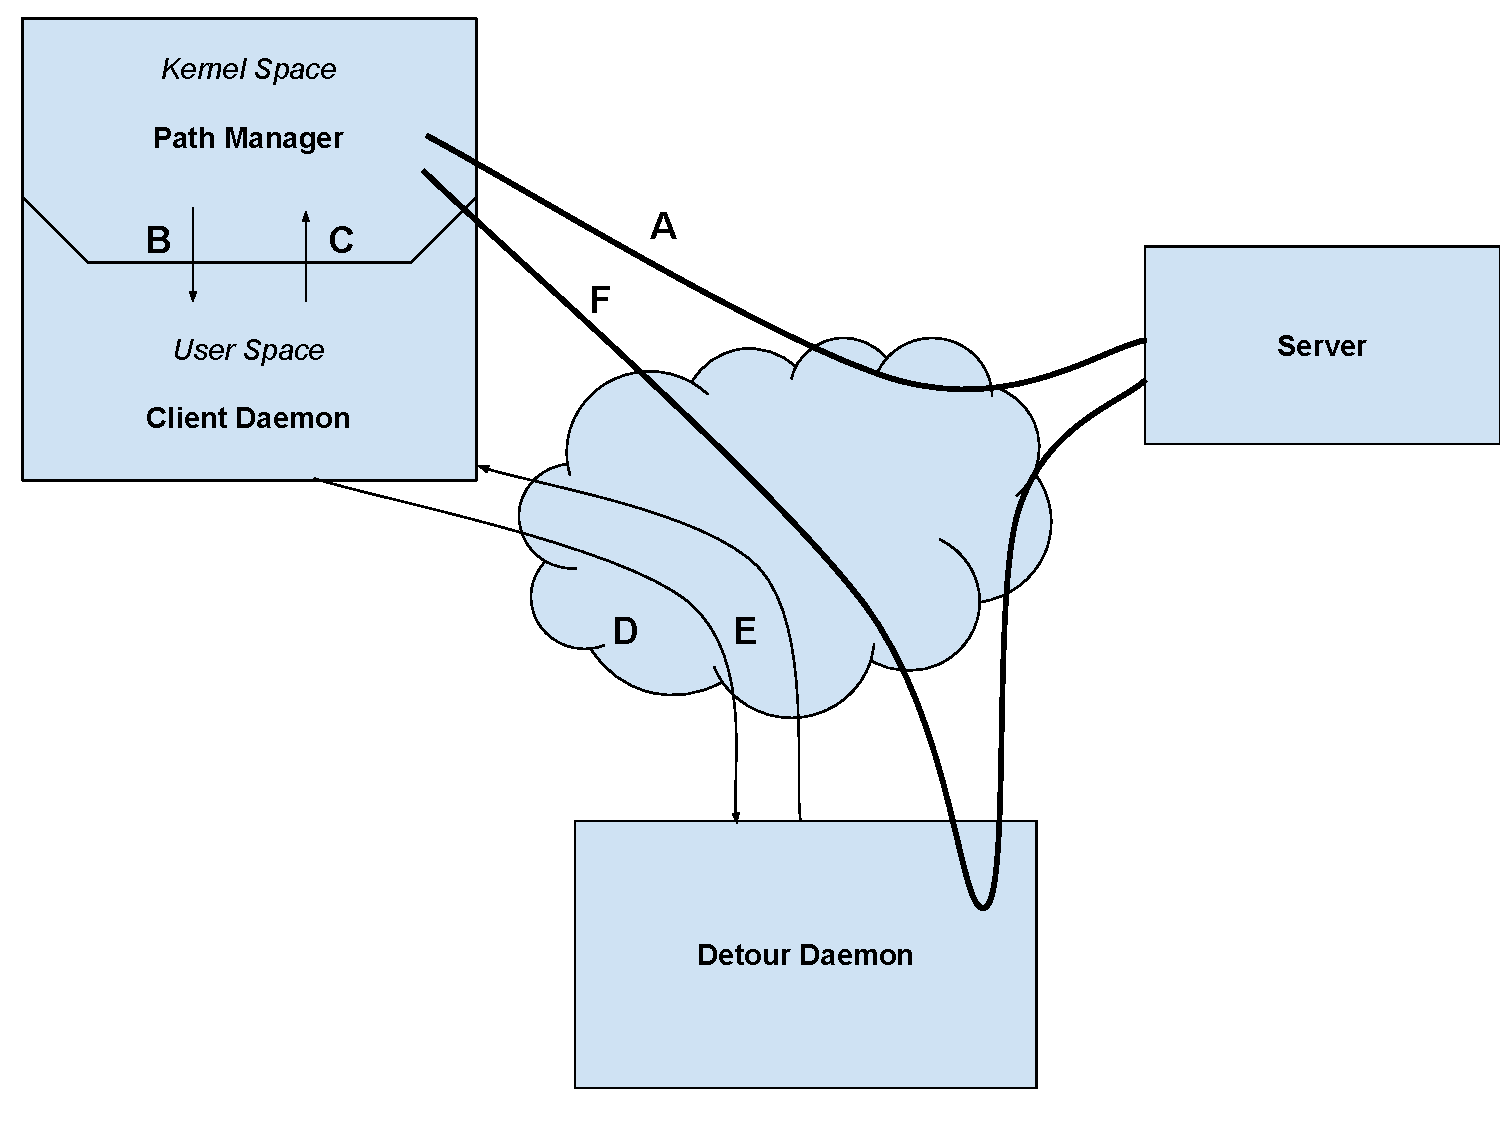
\includegraphics[width=0.8\textwidth]{figures/MovingParts.pdf}
  \caption[Interaction of client, detour, and server]{
    The components and their communications. In \textbf{A}, the path manager
    requests an overlay route. In \textbf{B}, the client daemon reports overlay
    routes back to the path managers. In \textbf{C} and \textbf{D}, the client
    and detour daemons negotiate an overlay route. In \textbf{E}, a subflow is
    created through the detour.
  }
  \label{f:MovingParts}
\end{figure}

The typical interaction of these components is as follows. First, a process on
the client creates a \ac{mptcp} connection to the server. The first subflow uses
the Internet routed path. Once this connection is fully established, the path
manager requests overlay routes on which it may create subflows. The client
detour daemon receives this request, and attempts to set up detours based on a
static configuration file. The client and detour daemons negotiate a tunnel,
which may be implemented in two different ways. The client reports this back to
the kernel, which creates subflows for the \ac{mptcp} connection across every
available detour, until a predefined limit is reached. In our implementation,
this limit is two, but it may be modified by a sysctl.

In the remainder of this chapter, we will discuss each of these components at
length.

\section{Detour Daemon}

We have implemented two different mechanisms for tunneling \ac{mptcp} subflows across
a detour. In both cases, the detour host must run a daemon that assists in
tunneling traffic from the client to the server.

\subsection{OpenVPN Tunneling}

The first mechanism involves the open-source tool OpenVPN
\cite{yonan2007openvpn}. OpenVPN is a program which provides virtual networking
between two computers. It comes with two operating modes. The first provides a
simple virtual link between two hosts, with no other capabilities. The second
uses this virtual link to create a virtual network. One host is the server,
which provides IP addresses and routes traffic among clients and the rest of the
Internet. OpenVPN also provides encryption and PKI-based authentication
services. Our detour runs OpenVPN as a server in the second mode of operation,
configured as follows:

\begin{itemize}
\item The connection is over UDP, to avoid the so-called ``TCP Meltdown'' effect
  caused by two sets of TCP timers and congestion control algorithms interfering
  with each other when TCP is tunneled through TCP \cite{khanvilkar2004virtual}.
\item The initial connection negotiation requires the client and server to
  exchange certificates.
\item Subsequent messages are not protected by encryption or signatures, to
  reduce per-packet space and time overhead.
\end{itemize}

Clients connect to this VPN, creating a virtual network device. The
client receives a routing rule from the detour advertising that it can reach all
hosts on the Internet with a very high cost. As a result, the client operating
system will prefer other routes instead of the VPN. However, the route is
available for the path manager to route subflows along.

One important aspect of VPN configuration is that the detour must create a
private IP subnet. It provides a DHCP service in order to assign IP addresses to
clients as they connect to the VPN. Clients are expected to be able to connect
to multiple detours simultaneously. In order to do this without conflict, each
detour must use a distinct private IP subnet, so that there is no chance of the
client addresses overlapping, and also so that the gateway address of the VPN is
unique on the client.

In a large-scale implementation of this technology, these subnet allocations
could be handled by a centralized detour management server. The 10.0.0.0/8
subnet is reserved for private networks, and if each detour were to establish
its own /24 subnet, there would be capacity for 65,536 non-conflicting subnets.
However, in our testing, subnets were manually allocated to avoid conflicts.

Finally, in order to forward VPN traffic to the internet, the detour must be
configured (via Netfilter) to perform network address translation (NAT) on
outgoing packets. This process is typical for a home router and for VPNs which
provide Internet access. As discussed earlier, \ac{mptcp} is designed with this
behavior in mind, and so it is capable of functioning through NAT, so long as
the middleboxes do not remove TCP options in transit, or modify data contents
\cite{rfc6182}.

The OpenVPN implementation has several attractive qualities. First, it relies on
a well-used protocol for forwarding traffic. Second, it need not be configured
on a per-connection basis. Finally, it provides a built in mechanism for
mutually authenticating the client and detour. However, there are some
drawbacks. Since packets are tunneled, at least 28 bytes of overhead (IP and UDP
headers) are required. To avoid fragmentation, the connection's maximum segment
size (MSS) may need to be adjusted, although in our testing, this was not
required.

\subsection{NAT Tunneling}

The second approach directly modifies packet source and destination addresses,
without actually using a protocol (like OpenVPN) for tunneling. Rather than
establish a generic tunnel with the detour, we instead inform the detour of our
intended destination, and request that it perform \ac{nat} on our packets. Then,
we address packets directly to the detour, on an agreed upon port. The detour
forwards these to the final destination, and forwards reply packets to the
client. In order to do this, clients use a simple signaling protocol to request
tunnels from a detour.

\begin{figure}
  \centering
  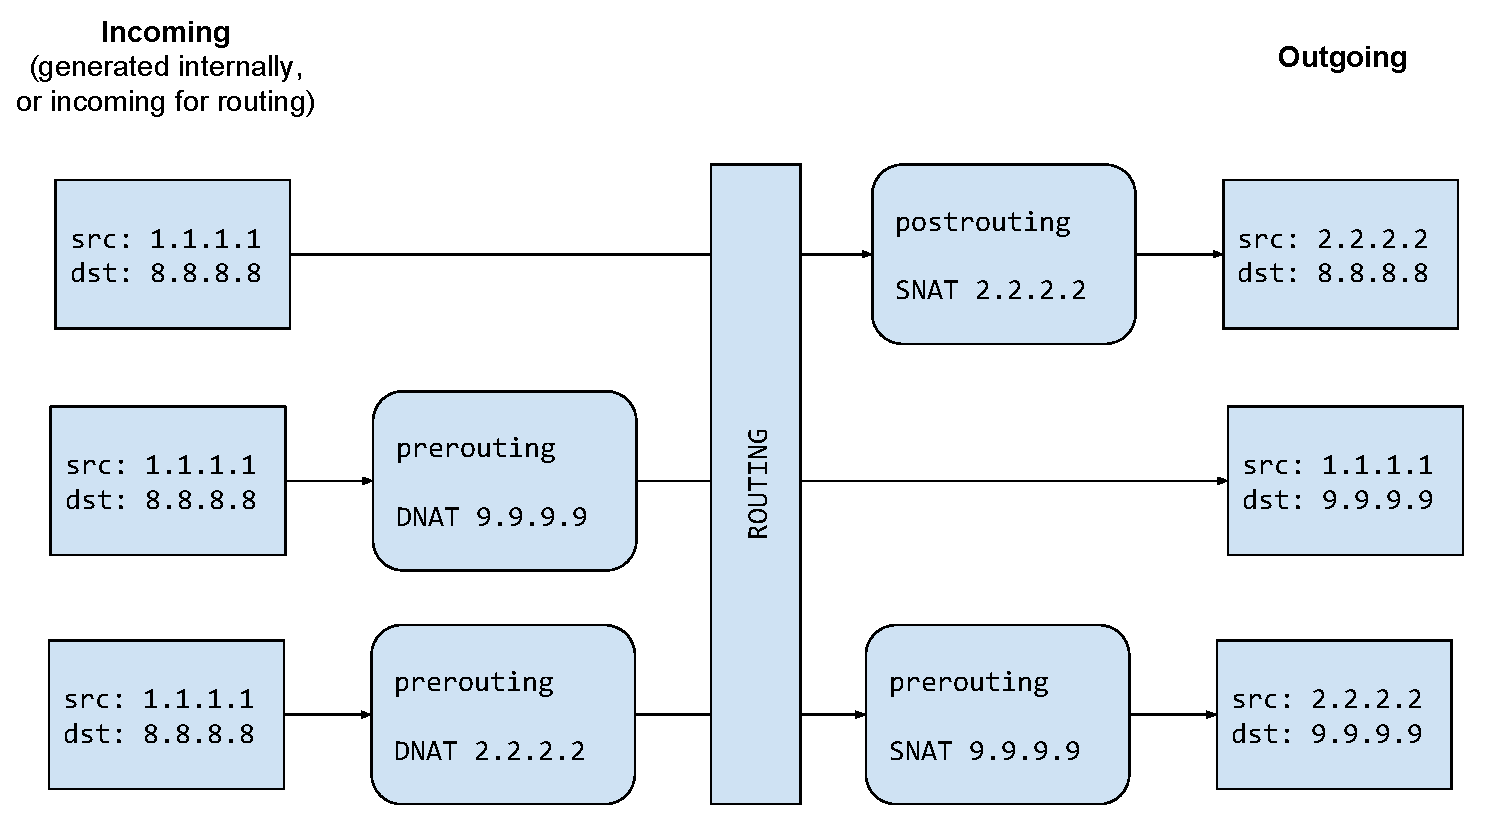
\includegraphics[height=0.3\textheight]{figures/NATTypes.pdf}
  \caption[Types of NAT provided by Netfilter]{Types of NAT provided by
    Netfilter. \textbf{Top:} SNAT only. \textbf{Middle:} DNAT only.
    \textbf{Bottom:} Both SNAT and DNAT, as used in the NAT tunnel.}
  \label{fig:NATTypes}
\end{figure}

The Linux kernel's Netfilter framework allows for two types of NAT, illustrated
in Figure~\ref{fig:NATTypes} \cite{russell2002nat}. The first kind, source NAT
(SNAT), rewrites the source address of the packet. This is the typical form of
NAT used by home routers: the source address of an outgoing connection is
rewritten to be the router's external IP address, but the destination is
unchanged. This type of rule is applied after routing has taken place. The
second kind of NAT supported by Netfilter is destination NAT (or DNAT) which
rewrites the destination of the packet. This rule is applied before routing, so
that a proper interface can be selected for the new address.

The detour takes advantage of both forms of NAT offered by the kernel. First, it
applies DNAT, setting the destination address to be the final server's IP
address (signaled ahead of time). Then, it applies SNAT, setting the source
address to be its own external IP. The Netfilter framework remembers these
connections so that reply packets are properly forwarded back to the client.

Thanks to Netfilter, this NAT mapping can be arranged with two \texttt{iptables}
commands, with no custom kernel or user-space code required for packet
forwarding. It is possible to implement this in userspace using Netfilter-Queue
and a user-space application, but this approach has several drawbacks. It would
have to be single-threaded, and it would require that packet data be copied from
kernel space into user space and back. More critically, the connection tracking
provided by the kernel is more robust than what would be implemented by user
space.

As mentioned earlier, the server address must be communicated to the detour
ahead of time in order to use this scheme. To that end, we have designed a
simple UDP-based protocol for clients to request NAT mappings from a detour. The
detour listens for requests on UDP port 45672. The request format is shown
in Figure~\ref{fig:udp-nat-packet}.

\begin{figure}
  \centering
\begin{BVerbatim}
+-----------------------------------+
| ver(1) | op(1)  | reserved (2)    |
+-----------------------------------+
|           rip (4 bytes)           |
+-----------------------------------+
| rpt (2 bytes)   | dpt (2 bytes)   |
+-----------------|-----------------+
\end{BVerbatim}
  \caption{UDP NAT tunnel request structure}
  \label{fig:udp-nat-packet}
\end{figure}

The \texttt{ver} field is a protocol version, currently set to 1. The
\texttt{op} field contains the operation of this message: request (0) or
response (1). The \texttt{reserved} field is unused, providing padding for the
request. In the future, this field could be used for flags that enable IPv6
support. Since there are several IP addresses and ports involved in the
tunneling setup, we will define them each before defining the remaining fields
of the message.

\begin{itemize}
\item Client IP, port: the IP address of the client, and the client-side port,
  which is usually ephemeral.
\item Detour IP, port (client side): the IP and port that the client will
  address its communication to.
\item Detour IP, port (remote side): the IP and port which are used when the
  detour opens its corresponding connection on the remote.
\item Remote IP, port: the IP and port which the client is tunneling its
  connection to.
\end{itemize}

The fields \texttt{rip} (short for ``remote IP'') and \texttt{rpt} correspond to
remote IP and port. The \texttt{dpt} field corresponds to the detour port,
client side. In a request, the client proposes a \texttt{dpt} (usually the same
as the \texttt{rpt}). In the response, the detour specifies the actual port
which should actually be. The detour may wish to alter the \texttt{dpt} field
for several reasons:

\begin{itemize}
\item A tunnel to the remote IP, port pair is already open. The detour may wish
  to return the \texttt{dpt} already associated.
\item The client is already using the given \texttt{dpt} to connect to a
  different remote IP and/or port.
\item The detour may have a socket listening for connections on the proposed
  port (such as an HTTP server on port 80), and so it may wish to avoid creating
  a tunnel which would prevent the client from accessing that service.
\end{itemize}

In order to create the tunnels, the detour runs two IPTables commands, which
create NAT rules. The first performs DNAT:

\begin{lstlisting}
iptables -t nat -A PREROUTING \
         -s (*\emph{ClientAddress}*) \
         -d (*\emph{DetourAddress}*) \
         -p tcp --dport (*\emph{DetourPort}*) \
         -j DNAT --to (*\emph{RemoteAddress}*):(*\emph{RemotePort}*)
\end{lstlisting}

In this command, we add to the \texttt{nat} table, on the \texttt{PREROUTING}
chain. Incoming packets from the client, addressed to the agreed upon
\textit{DetourPort} are sent to the \texttt{DNAT} chain, which rewrites the
destination address to be the agreed upon remote address and port. This must
occur before the kernel routes the packet. Once the kernel has routed the
packet, the DNAT rule can be applied:

\begin{lstlisting}
iptables -t nat -A POSTROUTING \
         -s (*\emph{ClientAddress}*) \
         -d (*\emph{RemoteAddress}*) \
         -p tcp --dport (*\emph{RemotePort}*) \
         -j SNAT --to (*\emph{DetourAddress})
\end{lstlisting}

Since the destination address and port have already been modified, this rule
looks for packets addressed to the remote address and port, but still using the
client address as the source. It jumps these packets to the DNAT chain, where
their source address will be rewritten as the detour's address.

It is important to understand that these rules are generally only applied to the
initial SYN segment of the TCP flows. Once these rules are applied, the
connection tracking mechanism of the kernel takes over, ensuring that these
rules are applied in reverse to response packets.

The detour daemon is implemented as a Python script. It listens for tunnel
requests, executes the correct commands to create them, and then sends
responses. It ensures that detour ports do not conflict with each other, or with
ports that are open on the daemon machine. It also ensures that on termination,
all tunnels are torn down.

This mechanism has the advantage that it requires zero space overhead within the
packet. Since no headers are added, the full amount of data may be transmitted
on these segments. However, its disadvantage is that tunnels must be configured
each time a new connection is created on the client. In the case of OpenVPN, a
new subflow may routed through an existing OpenVPN connection without any
additional communication with the detour. However, with the NAT approach, each
time a subflow is initiated with a new server, a tunnel must first be negotiated
with the detour server.

\section{Path Manager}

To enable subflows to use the detours created above, we implement a custom
\ac{mptcp} path manager within the Linux kernel. As previously described, the
path manager is a module which dictates local policy for creating new subflows
and announcing local addresses.

\begin{figure}
  \centering
  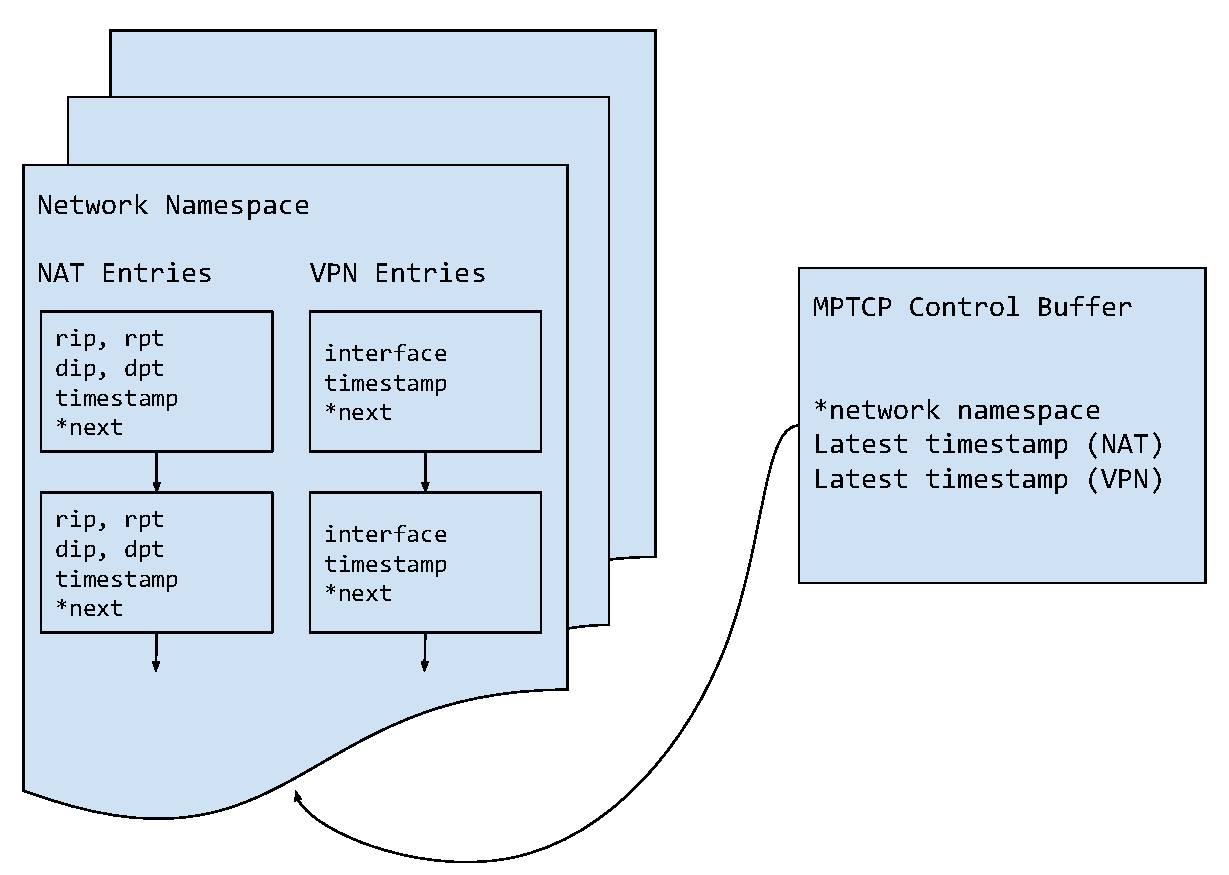
\includegraphics[width=0.8\textwidth]{figures/KernDataStruct.pdf}
  \caption{Simplified view of Path Manager data structures}
  \label{fig:KernDataStruct}
\end{figure}

The path manager receives space within the \ac{mptcp} control buffer in order to
track state, and it registers a set of callbacks with the protocol, so that it
can be notified of events as they occur. Global state, such as the list of
available detours, must be stored on a per-network namespace basis. This is
required not only to satisfy the demands of a modern kernel which supports
namespacing and containerization, but also so that experiments using Mininet,
which relies on namespaces, run successfully. A simplified view of the data
structures maintained by the path manager is presented in
Figure~\ref{fig:KernDataStruct}.

The path manager consists of two main components. First, a background worker
which selects and adds detours to \ac{mptcp} connections. Second, a
communication interface so that information and commands can be exchanged with
user-space components.

\subsection{Subflow Worker}

The subflow worker runs in two situations, in the context of a particular
\ac{mptcp} socket. First, when a \ac{mptcp} connection becomes fully established
(i.e. after the three-way handshake completes). Second, when a new detour has
been made available to this network namespace, and the detour could be used for
this connection.

On its first run, the subflow worker uses the Generic Netlink communication
interface (described in Section~\ref{s:genl}), requesting a detour. Then, it
looks through an internal list of detours. The kernel maintains two lists of
detours (per network namespace). The first is a list of OpenVPN detours. These
detour entries are not specific to a server, and they simply indicate the name
of a network interface to use. The second list contains NAT detours. These
consist of a detour address and port, and a server address and port. The worker
may only select NAT entries which match the destination address and port of the
connection it is working on.

The task attempts to add up to $N$ subflows, where $N$ is a configurable limit.
It terminates in one of two ways. Either it has exhaused all of the available
detours, but not yet created all $N$ subflows. Otherwise, if it creates $N$
subflows successfully, it stops looking through the list, even if more detours
are available. If OpenVPN detours are available, then they take precedence over
the NAT detours, because they are available immediately. NAT detours created by
the client daemon become available only once the daemon has processed the
request from the kernel.

\subsection{Generic Netlink}
\label{s:genl}

In order to request and receive detour entries from userspace, the path manager
relies on a communication interface based on Generic Netlink. Netlink is an
address family for the socket interface (\texttt{AF\_NETLINK}, similar to
\texttt{AF\_INET}), which allows communication between kernel and userspace.
Many existing Linux network configuration utilities communicate with the kernel
over the Netlink address family, such as route and firewall configuration. Each
of the subsystems being configured has a corresponding protocol family, such as
\texttt{NETLINK\_NETFILTER} for Netfilter firewall configuration. These protocol
families take the same place in the \texttt{socket()} system call as protocol
families such as \texttt{IPPROTO\_TCP} in the \texttt{AF\_INET} and
\texttt{AF\_INET6} address families.

Creating a new Netlink protocol would involve allocating a new Netlink protocol
family. To make this process easier, the Generic Netlink protocol family was
created. It allows custom protocols (``Generic Netlink families'') to be
created, dynamically allocated, and discovered. It also provides a common format
for sending several data types, and creates a framework for defining message
types. Further, Generic Netlink provides a multicast capability, allowing kernel
and user sockets to broadcast messages to any socket which has joined a
particular multicast group. Finally, Generic Netlink comes with a kernel and
userspace library which allows for a consistent API and a level of abstraction
when defining Generic Netlink families.

We implement a Generic Netlink family, with the following operations
implemented:

\begin{itemize}
\item \texttt{DETOUR\_C\_REQ}: An announcement message sent from the kernel to a
  multicast group, which the client daemon subscribes to. Specifies a remote
  address and port which the kernel would like to create a detour to.
\item \texttt{DETOUR\_C\_ADD}: A command sent from userspace to the kernel. Adds
  a detour (of type NAT or VPN) to the kernel's internal list of detours. When a
  new, unique detour is received, this command looks through each connection in
  the current network namespace and wakes its worker, so it may consider using
  the detour.
\item \texttt{DETOUR\_C\_DEL}: A command sent from userspace to the kernel.
  Removes a detour from the kernel's internal list.
\item \texttt{DETOUR\_C\_ECHO}: A command sent from userspace to the kernel,
  requesting that the kernel write out its list of detours to the kernel log.
  This is a useful command for development and debugging.
\end{itemize}

Generic Netlink provides mechanisms for giving permissions to each operation,
and allows the kernel to work only within the network namespace of the calling
program. As a result, the client daemon may only add or remove detours or
receive requests from its own namespace.

\section{Client Daemon}

The client daemon has two main responsibilities. First, it must create OpenVPN
connections and report them to the kernel. Second, it must respond to detour
requests from the kernel by creating NAT detours and reporting them back.

The daemon has a configuration file which allows the user to specify the IP
addresses of hosts to use for both types of detours. On startup, the daemon
executes the OpenVPN client software, and waits for it to fully initialize. A
new thread is used to monitor the OpenVPN client process, logging any important
messages.

Next the daemon creates a UDP socket corresponding to each NAT detour in its
configuration file. A separate thread is launched, which calls \texttt{select()}
on the set of detour sockets, waiting for incoming responses from any detour.

Finally, the detour creates a Netlink socket, subscribes to the path manager's
multicast group, and begins waiting for requests. For each request, it sends a
UDP request to every NAT detour. When the receiving thread receives a response,
it sends the final data over the Netlink socket back to the path manager.

\section{Security Considerations}

Using this mechanism, a malicious third-party detour could be given access to
read and modify the partial contents of an \ac{mptcp} connection. We believe
that this risk is mitigated by the following factors:

\begin{itemize}
\item Usage of TLS, especially in the web, is becoming ubiquitous. Due to the
  design of our \ac{mptcp} and our system, the initial three-way handshake of
  TCP is completed before any subflows can begin initialization. TLS handshake
  information will thus be exchanged on the first subflow, before or
  concurrently with the establishment of additional subflows. As a result,
  connections can be protected by TLS by the time additional subflows are
  transmitting data. TLS encrypts data, protecting the privacy of the
  transmission, and detects modifications, preventing modification of data by a
  malicious detour.
\item Modifications of data that result in changing the \ac{dss} mapping size
  are likely to be detected and treated as a \ac{mptcp} protocol error.
\item A large-scale implementation of this mechanism could involve mutual
  authentication of the client and detour, via PKI. So long as a third party can
  be trusted to verify that a detour is malicious, and the third party can be
  trusted, a scheme like this can prevent malicious third-parties from being
  used as detours.
\end{itemize}

\chapter{Evaluation}
\label{c:eval}

The literature has already established that one-hop overlay routes can improve
connection latency, loss rate, and throughput
\cite{detour,ron,gummadi2004improving}. Therefore, when designing experiments to
evaluate our system, we did not attempt to replicate these results. Instead, we
attempted to answer the following questions:

\begin{itemize}
\item Given a network where an alternative path with better connection
  properties exists, can this mechanism effectively use the alternative path?
\item Given a network where the core is the bottleneck, rather than access
  links, can this method aggregate the throughput of alternative paths?
\item Can this mechanism be used effectively on the wide area Internet?
\end{itemize}

We design two types of experiments to answer each of these questions. The first
is based on network emulation, and is designed to answer the first two questions
regarding specific network topologies. The second experiment deploys this
mechanism across geographically distributed hosts, to evaluate the performance
and deployment potential on the wide area Internet.

\section{Mininet Experiments}

Our first set of experiments are based on the Mininet tool \cite{mininet}.

\subsection{Fidelity Considerations}

One criticism of the Mininet framework is that in situations with high load, its
performance fidelity can suffer \cite{lantz2010network}. Later work has
addressed this by allowing users to limit the CPU utilization of each emulated
host, as well as restricting the bandwidth of links using the Linux traffic
control features \cite{handigol2012reproducible}.

We observed that our test systems could emulate networks with throughput up to
24 Gbps. To ensure that our experiments did not approach the limits of Mininet's
performance fidelity, we limited the bandwidth of each link to no more than
20Mbps, and used relatively few hosts and links. Each host is CPU limited, so
that it may use no more than a tenth of the available processor time. Finally,
we used experiment output provided by IPerf to verify that CPU utilization
remained low during each experiment. In all cases, CPU utilization was no higher
than 5\% over the course of an experiment.

\subsection{Topology}

\begin{figure}
  \centering
  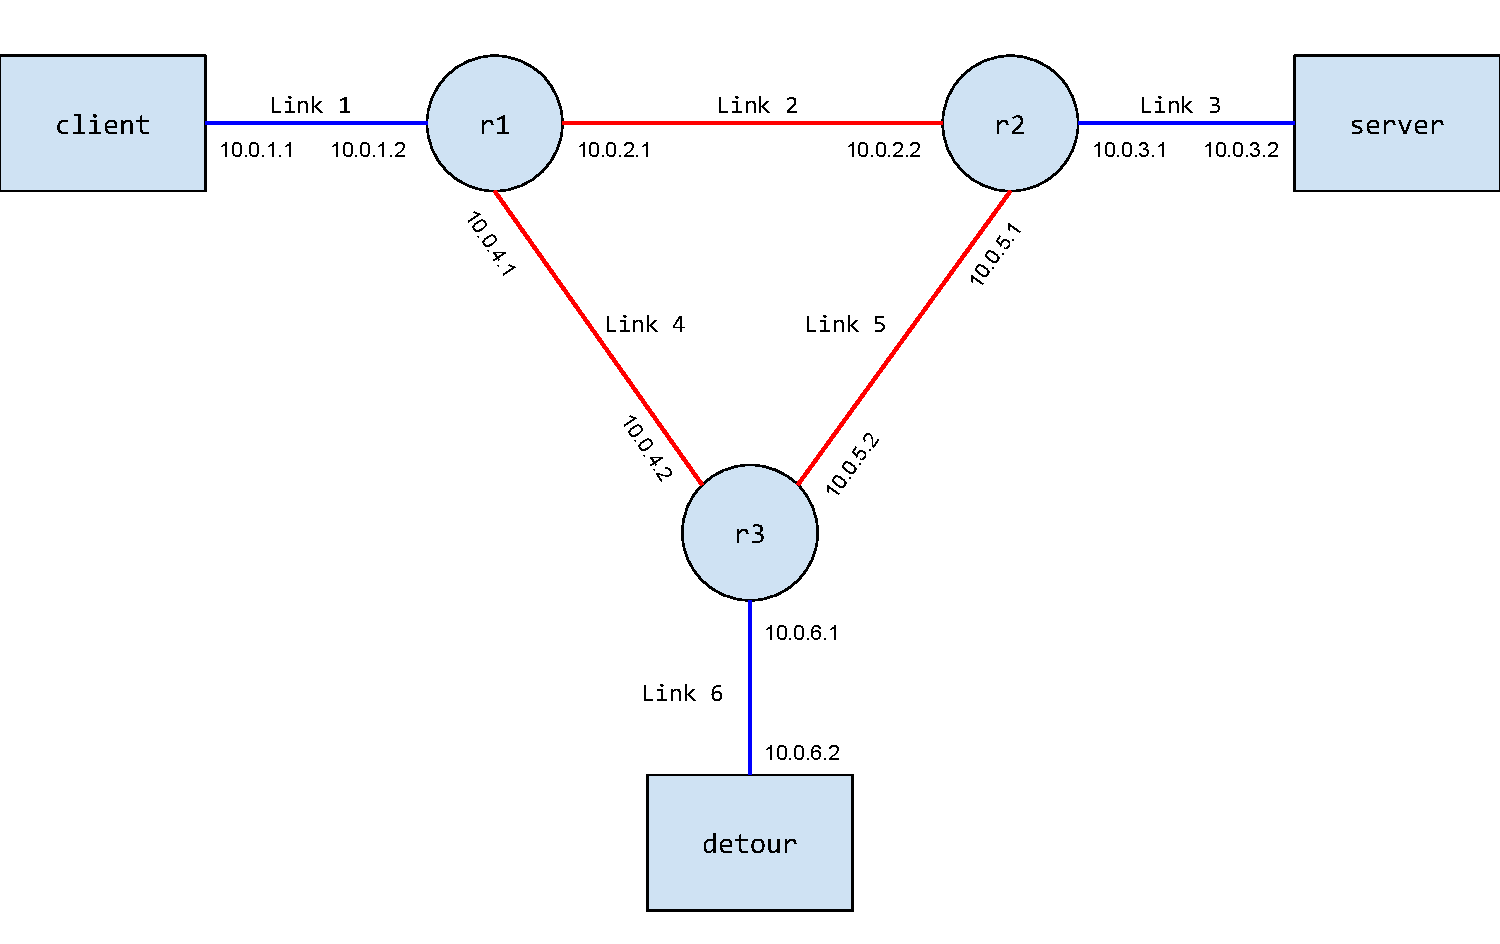
\includegraphics[width=\textwidth]{figures/Topology.pdf}
  \caption{Experimental network topology}
  \label{fig:topo}
\end{figure}

Our network topology is illustrated in Figure~\ref{fig:topo}. The routers
\texttt{r1} through \texttt{r3} are Linux hosts, as described in the previous
section. They are statically configured with routes, so that the default route
from \texttt{client} to \texttt{server} traverses Link 2. Routing is enabled,
and all routing occurs within the kernel.

While configuring routing tables, we encountered issues where Linux kernel
routing rejected incoming packets as ``Martians.'' That is, packets which
originated from an interface which is not the default route for their source
address. To avoid these issues, we disabled Martian filtering in the Linux
kernel.

\subsection{Methodology}

To evaluate the performance of this mechanism, we vary the traffic control
configurations of the links in the topology. There are two main traffic control
configurations tested.

\begin{itemize}
\item \textbf{Symmetric.} The first configuration gives each link the same
  traffic control properties: 10Mbps bandwidth and 5ms delay.
\item \textbf{Core-limited.} The second configuration gives each link within the
  network ``core'' (i.e. links 2, 4, and 5) 10Mbps of bandwidth and a 5ms delay.
  Meanwhile, the access links (i.e. links 1, 3, and 6) are assigned 20Mbps, with
  the same 5ms delay. This aims to provide a simplified configuration in which
  the access link can support more bandwidth than the default Internet path.
\end{itemize}

For each traffic control configuration, we also create two modifications.

\begin{itemize}
\item \textbf{Lossy.} Link 2 is configured to drop packets independently and
  randomly with probability 0.01.
\item \textbf{Delayed.} Link 2 is configured to have a high (100ms) latency.
\end{itemize}

This results in a total of six traffic control configurations. For each traffic
control configuration, we use the standard IPerf 3 tool to measure \ac{mptcp} or
TCP throughput between \texttt{client} and \texttt{server}. We test the
following configurations:

\begin{itemize}
\item \textbf{1-Subflow.} MPTCP is enabled, but no detours are configured on the
  client. The connection uses only one subflow, across the Internet routed path.
\item \textbf{NAT.} In addition to a subflow on the Internet routed path, a
  second subflow is through a NAT detour.
\item \textbf{OpenVPN.} In addition to a subflow on the Internet routed path, a
  second subflow is through a OpenVPN detour.
\item \textbf{TCP.} MPTCP is disabled. A regular TCP flow is used, across the
  default Internet routed path. The default Linux congestion control (CUBIC) is
  used.
\item \textbf{NAT TCP.} A regular TCP flow is used, but it is directed through
  the same NAT proxy mechanism used in the \textbf{NAT} configuration.
\item \textbf{OpenVPN TCP.} A regular TCP flow is used, but it is directed
  through the same OpenVPN proxy mechanism used in the \textbf{OpenVPN}
  configuration.
\end{itemize}

The throughput is measured with IPerf for a total of 60 trials for each
combination of traffic control and connection configuration. A trial consists of
a ten-second IPerf session.

\subsection{Results}

\begin{figure}
  \centering
  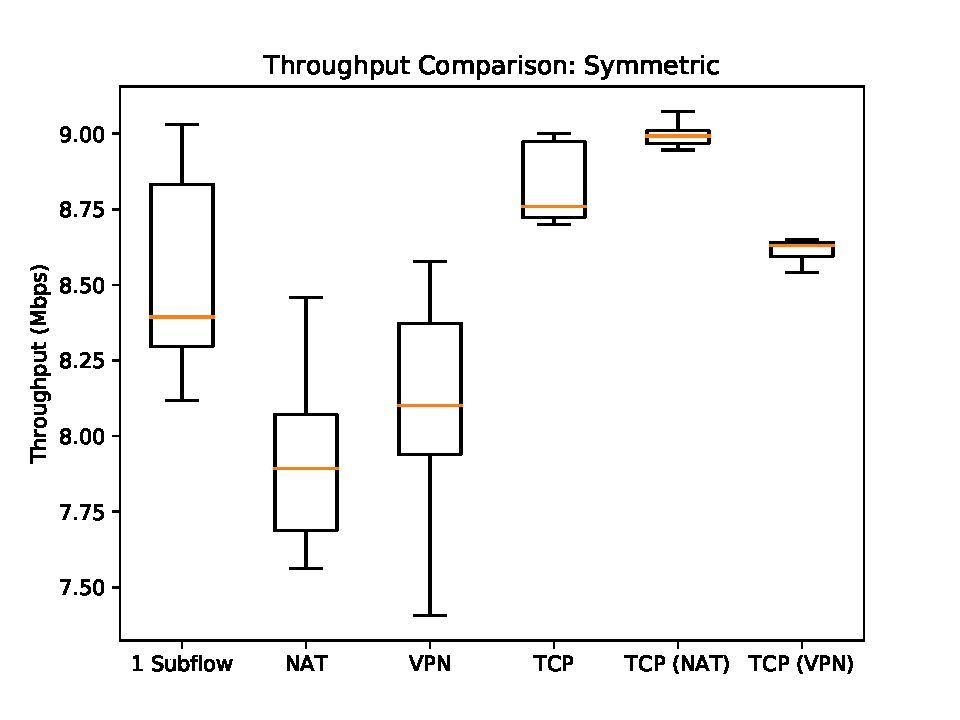
\includegraphics[height=0.45\textheight]{figures/sym.pdf}
  \caption{Throughput Comparison: Symmetric}
  \label{fig:sym}
\end{figure}

Figure~\ref{fig:sym} shows a performance comparison of the mechanism on the
Symmetric network without loss or latency. In this comparison, we can see three
important conclusions. First, splitting the traffic across two paths when the
bottleneck is shared results in more overhead and lower throughput. Second,
\ac{mptcp} with a single subflow shows more variable throughput behavior than
regular TCP. Third, regular TCP over the NAT detour demonstrates slightly higher
throughput than regular TCP over the VPN, although the difference is small (0.5
Mbps).

\begin{figure}
  \centering
  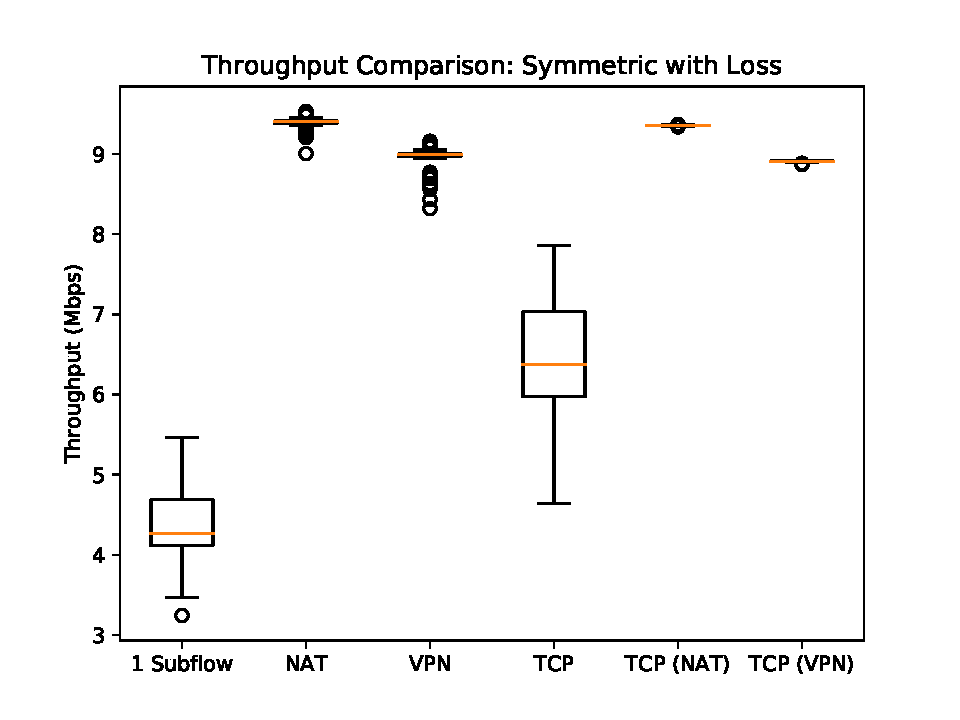
\includegraphics[height=0.45\textheight]{figures/sym-lossy.pdf}
  \caption{Throughput Comparison: Symmetric, with Loss}
  \label{fig:sym_lossy}
\end{figure}

In Figure~\ref{fig:sym_lossy}, we see the effect of adding a 1\% loss rate to
a link that is present only on the default path. Regular TCP and \ac{mptcp} with
one subflow show significant losses in throughput, although \ac{mptcp} is much
worse. When NAT or VPN paths are added to the \ac{mptcp} connection, the
performance is comparable to regular TCP traveling solely across those paths,
but no better.

\begin{figure}[p]
  \centering
  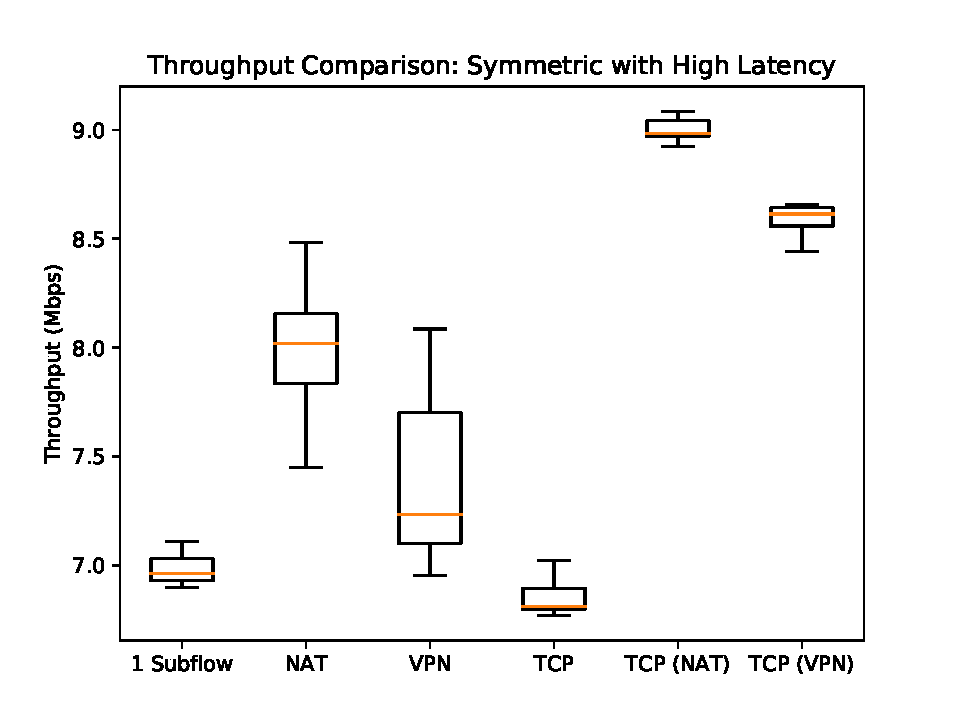
\includegraphics[height=0.42\textheight]{figures/sym-delayed.pdf}
  \caption{Throughput Comparison: Symmetric, with Latency}
  \label{fig:sym_delayed}
\end{figure}

\begin{figure}[p]
  \centering
  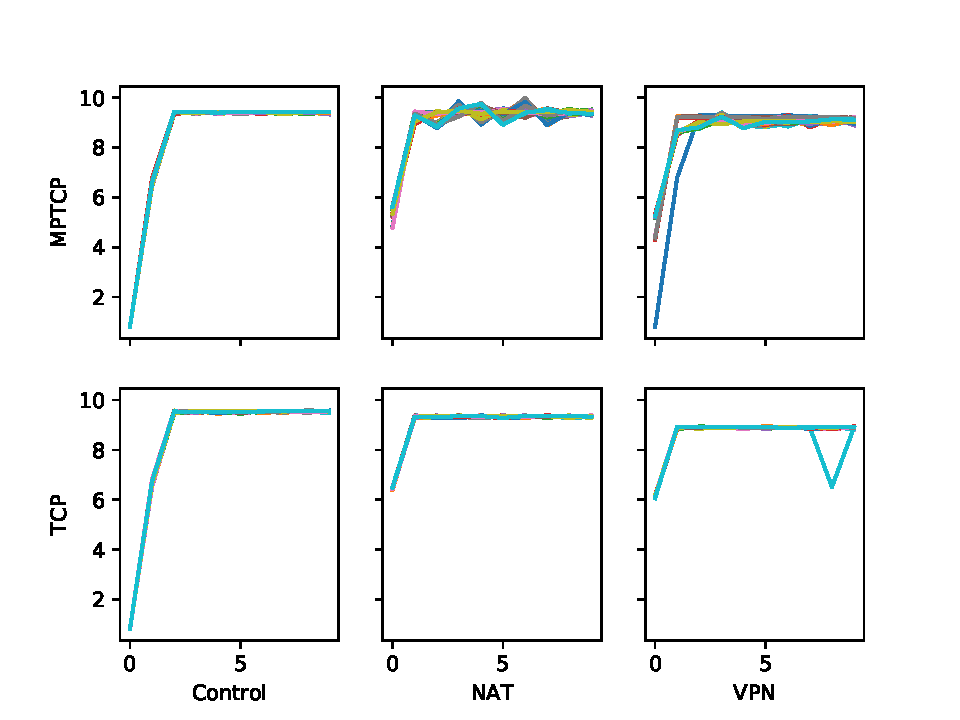
\includegraphics[height=0.42\textheight]{figures/timegrid-sym-delayed.pdf}
  \caption[Throughput Over Time: Symmetric, with Latency]{Throughput Over Time:
    Symmetric, with Latency. Units are Mbps on the y-axis and seconds along the
    x-axis.}
  \label{fig:timegrid_sym_delayed}
\end{figure}

In Figure~\ref{fig:sym_delayed}, we see the impact of the high latency link
along the default route. While it appears that there could be a somewhat
significant difference between the throughput, this is not the case.
Figure~\ref{fig:timegrid_sym_delayed} shows the throughput over time for
each of the experiments. Each of the experiments reaches nearly the same steady
state throughput, but at different times. This is most likely explained by the
different congestion control mechanisms used (CUBIC for regular TCP, versus the
Linked Increases algorithm used by \ac{mptcp}).

\begin{figure}[p]
  \centering
  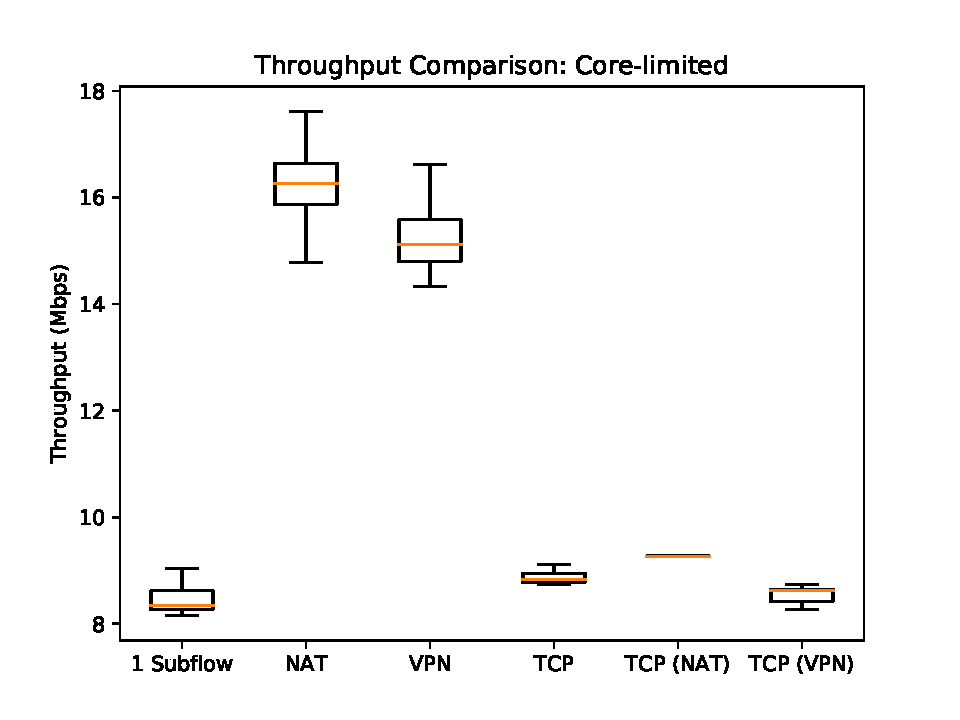
\includegraphics[height=0.45\textheight]{figures/easy.pdf}
  \caption{Throughput Comparison: Core-limited}
  \label{fig:easy}
\end{figure}

\begin{figure}[p]
  \centering
  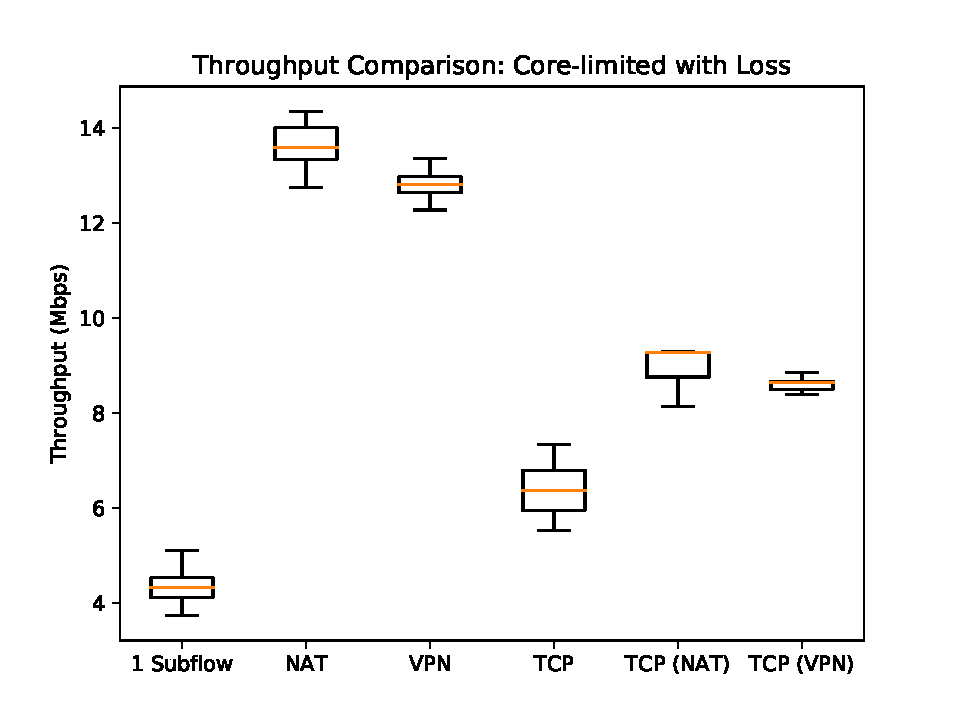
\includegraphics[height=0.45\textheight]{figures/lossy.pdf}
  \caption{Throughput Comparison: Core-limited, with Loss}
  \label{fig:lossy}
\end{figure}

The results for the core-limited network are much different.
Figure~\ref{fig:easy} shows a comparison of throughput on the core-limited
network, with no loss or latency. Since the detour path traverses different core
links than the default path, there is no competition. Thus there is the
potential to aggregate the capacity of both paths. Both the NAT and VPN methods
are able to aggregate nearly all of the capacity, although the NAT performs very
slightly better.

When loss is introduced, Figure~\ref{fig:lossy} shows that the NAT and VPN
methods outperform their pure TCP variants, since they are able to aggregate the
throughput of both paths. Even though the default path is lossy, it is able to
contribute some throughput to the \ac{mptcp} connection.

\subsection{Summary}

By emulating a network with varying conditions, we were able to examine how this
mechanism can aggregate throughput in different situations. When the mechanism
is used in a network with no traffic quality issues and no potential for
aggregation, there is a modest overhead. In a similar network with poor
connection characteristics along the default path, the mechanism is capable of
achieving throughput similar to a single flow across an alternative path.
When the network has potential for aggregation, the mechanism is capable if
aggregating nearly all of the available throughput. This results in better
performance than a single flow across any available path.

Across all the connections, the NAT approach performs slightly better than the
VPN, likely due to the additional overhead of the IP and UDP encapsulation,
along with any OpenVPN protocol overhead.

\section{AWS Experiment}

The Mininet experiments demonstrate that this method can indeed circumvent lower
quality paths, and also aggregate the capacity of different paths through the
network. However, these experiments run on a single platform: client, server,
detour, and routers all share the same network stack. The real Internet is much
more heterogeneous. To demonstrate the feasibility of this mechanism on the wide
area Internet, we designed a full-scale experiment.

Using Amazon Web Services' Elastic Cloud Compute service (AWS EC2), we deployed
three instances, each in a different region. The client is located in the
\texttt{us-west-1} region (Northern California), the detour in
\texttt{us-east-2} (Ohio), and the server in \texttt{us-east-1} (Northern
Virginia). We then ran the IPerf 3 tool for 100 trials in each of the following
configurations: \textbf{1-Subflow}, \textbf{NAT}, and \textbf{OpenVPN}.

\begin{figure}
  \centering
  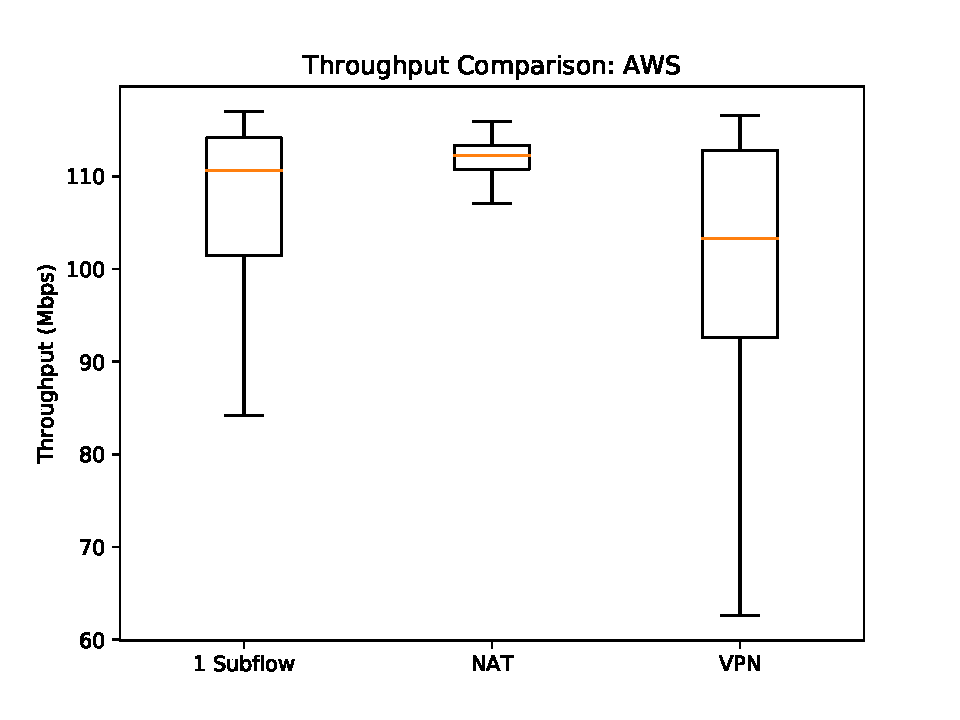
\includegraphics[height=0.45\textheight]{figures/aws.pdf}
  \caption{Throughput Comparison: AWS}
  \label{fig:aws}
\end{figure}

Figure~\ref{fig:aws} shows a comparison of the throughput for each of these
connections. It is clear from this figure that adding a detour was not effective
in improving throughput. However, it is clear that our mechanism is capable of
functioning on the wide-area Internet, at higher transmission rates than we
emulated in the Mininet experiments.

Another interesting result of this experiment is that the OpenVPN mechanism,
which performed slightly worse than the NAT mechanism in our Mininet tests,
slightly outperforms the NAT mechanism. Due to the wide variability in the data,
it is not clear whether this result is due to noise or due to an underlying
aspect of the mechanism.

\chapter{Future Work}
\label{c:fw}

The mechanism described here is complete, but has the potential for improvement
in several avenues. In this chapter, we describe several possible avenues for
continued work and research.

\section{Detour Collective}

One fundamental question regarding the deployment of this mechanism has not yet
been addressed: where are detour hosts found, and what is their motivation for
forwarding traffic? One possibility is that a group of users could form a group
that aims to help each other improve their connection quality. Some form of
protocol, either centralized or decentralize, could allow users to join,
offering their computer as a detour, in return for the use of other detour
hosts.

Ultimately, this group would be very similar to the overlay networks described
previously. However, unlike most of these, the overlay network would be
restricted to single hop source routing of \ac{mptcp} connections.

The VPN detouring mechanism would be particularly conducive to such a
collective. The OpenVPN protocol uses a PKI for authentication of client and
server. So, a centralized collective could use this PKI to enforce membership
cryptographically. When a user joins, they generate a private key and request
that the central authority sign it. By using the central authority's certificate
as a PKI root, they may ensure that only members of the collective could use
their detouring services. By having their private key signed, users could gain
access to the detouring services of other members.

\section{Dynamic Source Routing}

In the \ac{ron} system, overlay routing is performed at each node \cite{ron}.
Similarly, the Detour study describes a system in which routing is performed at
each overlay node \cite{detour}. In this system, we apply source routing. While
overlay routing mechanisms have been described for systems like \ac{ron} and
Detour, we are unaware of algorithms which attempt to find the best route for a
packet from its source, with incomplete knowledge of the capacity and state of
the network links.

An interesting extension to this work would be to extend it with such an
algorithm. This algorithm would maintain several \ac{mptcp} subflows, and every
so often it would decide to close one in favor of a new route. This decision
would have to take into account at least the following factors:

\begin{itemize}
\item RTT and observed loss rate of the subflow considered for eviction.
\item Change in RTT and observed loss rate of the other subflows since this one
  was added.
\item Potentially outside observations, such as statistics from other subflows,
  or statistics generated from userspace monitoring programs.
\end{itemize}

Together with a Detour Collective, this could almost completely automate the
process of using this framework for an end user.

\section{Data Scheduling}

The kernel modifications of this framework currently only consist of a path
manager. We have no control of the scheduling of data across the subflows we've
created, beyond selecting an appropriate scheduler. An extension of this work
could be to implement a data scheduler for the framework. A custom scheduler
could send data redundantly across new subflows just after they are added, so
that there is no loss in reliability when assessing the performance of a new
subflow. Further, a scheduler could detect whether a particular flow is
application limited or network limited, and schedule differently based on this.
For instance, redundantly sending data across each subflow could improve overall
latency and loss rates, but it would only make sense when the connection is
application limited. A network limited connection would be best served by a less
wasteful strategy, such as the default Lowest RTT First scheduler.

\section{IP Options}

Currently, the NAT forwarding mechanism uses a UDP-based protocol for requesting
tunnels. As a result, there is a one RTT overhead before each NAT detour may be
established. However, the NAT tunnel has lower overhead than the VPN method, and
thus performs measurably better. Removing the one RTT delay could make the NAT
method the best overall choice.

It may be possible to embed the final destination of the initial \texttt{SYN}
packet into an IP option. This would eliminate the need for a signaling
protocol. This would require implementing a Netfilter module for the detour
host's kernel.

\chapter{Conclusion}
\label{c:conclusion}

In this thesis, we have described the implementation and evaluation of a system
for adding non-default paths to \ac{mptcp} connections. We implemented this as a
path manager in the 0.91 version of the Multipath TCP Linux kernel, along with
several user-space utilities which complete the system.

The implementation is structured so that two different mechanisms for tunneling
subflows are allowed. We have seen that the NAT approach has slightly better
performance due to its lower per-packet overhead. However, that increased
performance comes at the expense of an extra RTT for setting up a tunnel, and
the extra complexity of a dynamic client which creates them. The VPN approach is
simpler, but has higher overhead.

When compared to standard TCP over the best available path, this mechanism
incurs a modest overhead when the same bottleneck link is present on both paths.
However, when the paths have separate bottlenecks, this mechanism is capable of
aggregating the bandwidth of both paths, achieving better performance than
standard TCP across the best path.

This mechanism is compatible with the wide area Internet today. We believe that
as high-bandwidth access links become more common, the collaborative bandwidth
sharing systems this enables will become more relevant. In the meantime, there
are several opportunities for extending this work and using it to study problems
like detour routing.

\backmatter
\appendix

\bibliographystyle{ieeetr}
\bibliography{paper}

\end{document}
